\documentclass[12pt, a4paper, twoside]{scrartcl}
 %---- Allgemeine Layout Einstellungen ------------------------------------------

% Für Kopf und Fußzeilen, siehe auch KOMA-Skript Doku
\usepackage[komastyle]{scrpage2}
\pagestyle{scrheadings}
\setheadsepline{0.5pt}[\color{black}]


%Einstellungen für Figuren- und Tabellenbeschriftungen
\setkomafont{captionlabel}{\sffamily\bfseries}
\setcapindent{0em}


%---- Weitere Pakete -----------------------------------------------------------
% Die Pakete sind alle in der TeX Live Distribution enthalten. Wichtige Adressen
% www.ctan.org, www.dante.de

% Sprachunterstützung
\usepackage[ngerman]{babel}

% Benutzung von Umlauten direkt im Text
% entweder "latin1" oder "utf8"
\usepackage[utf8]{inputenc}

% Pakete mit Mathesymbolen und zur Beseitigung von Schwächen der Mathe-Umgebung
\usepackage{latexsym,exscale,stmaryrd,amssymb,amsmath}

% Weitere Symbole
\usepackage[nointegrals]{wasysym}
\usepackage{eurosym}

% Anderes Literaturverzeichnisformat
%\usepackage[square,sort&compress]{natbib}

% Für Farbe
\usepackage{color}

% Zur Graphikausgabe
%Beipiel: \includegraphics[width=\textwidth]{grafik.png}
\usepackage{graphicx}

% Text umfließt Graphiken und Tabellen
% Beispiel:
% \begin{wrapfigure}[Zeilenanzahl]{"l" oder "r"}{breite}
%   \centering
%   \includegraphics[width=...]{grafik}
%   \caption{Beschriftung} 
%   \label{fig:grafik}
% \end{wrapfigure}
\usepackage{wrapfig}

% Mehrere Abbildungen nebeneinander
% Beispiel:
% \begin{figure}[htb]
%   \centering
%   \subfigure[Beschriftung 1\label{fig:label1}]
%   {\includegraphics[width=0.49\textwidth]{grafik1}}
%   \hfill
%   \subfigure[Beschriftung 2\label{fig:label2}]
%   {\includegraphics[width=0.49\textwidth]{grafik2}}
%   \caption{Beschriftung allgemein}
%   \label{fig:label-gesamt}
% \end{figure}
\usepackage{subfigure}

% Caption neben Abbildung
% Beispiel:
% \sidecaptionvpos{figure}{"c" oder "t" oder "b"}
% \begin{SCfigure}[rel. Breite (normalerweise = 1)][hbt]
%   \centering
%   \includegraphics[width=0.5\textwidth]{grafik.png}
%   \caption{Beschreibung}
%   \label{fig:}
% \end{SCfigure}
\usepackage{sidecap}
\usepackage{float}

% Befehl für "Entspricht"-Zeichen
\newcommand{\corresponds}{\ensuremath{\mathrel{\widehat{=}}}}
\newcommand{\folgt}{\ensuremath{\mathrel{\Rightarrow}}}
\newcommand{\equals}{\ensuremath{\mathrel{\Leftrightarrow}}}
\newcommand{\degree}{\ensuremath{\mathrel{^{\circ}}}}

\newcommand{\nn}{\nonumber}
\newcommand{\tn}[1]{\textnormal{#1}}
\newcommand{\D}{\ensuremath{\mathrel{\rm d}}}

\newcommand{\const}{\tn{const}}

\newcommand{\meter}{\ensuremath{\mathrel{\tn m}}}
\newcommand{\kilogramm}{\ensuremath{\mathrel{\tn{kg}}}}
\newcommand{\second}{\ensuremath{\mathrel{\tn s}}}
\newcommand{\sekunde}{\second}

\newcommand{\volt}{\ensuremath{\mathrel{\tn V}}}
\newcommand{\pascal}{\ensuremath{\mathrel{\tn{Pa}}}}
\newcommand{\coulomb}{\ensuremath{\mathrel{\tn C}}}
\newcommand{\newton}{\ensuremath{\mathrel{\tn N}}}
\newcommand{\liter}{\ensuremath{\mathrel{\tn l}}}
\newcommand{\celsius}{\ensuremath{\mathrel{\tn C}}}
\newcommand{\fahrenheit}{\ensuremath{\mathrel{\tn F}}}
\newcommand{\joule}{\ensuremath{\mathrel{\tn J}}}
\newcommand{\kelvin}{\ensuremath{\mathrel{\tn K}}}
\newcommand{\mol}{\ensuremath{\mathrel{\tn{mol}}}}
\newcommand{\gramm}{\ensuremath{\mathrel{\tn{g}}}}

\newcommand{\kilo}{\ensuremath{\mathrel{\tn k}}}
\newcommand{\hecto}{\ensuremath{\mathrel{\tn h}}}

\newcommand{\centi}{\ensuremath{\mathrel{ \tn c}}}
\newcommand{\milli}{\ensuremath{\mathrel{ \tn m}}}
\newcommand{\micro}{\ensuremath{\mathrel{ \tn\mu }}}



%\newcommand{}{\ensuremath{\mathrel{  }}}
%\newcommand{}{\ensuremath{\mathrel{  }}}
%\newcommand{}{\ensuremath{\mathrel{  }}}


\newcommand{\person}[1]{\textsc{#1}}

 \begin{document}
 %Titelseite
\begin{titlepage}
\centering
\textsc{\Large Anfängerpraktikum der Fakultät für
  Physik,\\[1.5ex] Universität Göttingen}

\vspace*{4.2cm}

\rule{\textwidth}{1pt}\\[0.5cm]
{\huge \bfseries
  Spezifische Wärme der Luft und Gasthermometer}\\[0.5cm]
\rule{\textwidth}{1pt}

\vspace*{3.5cm}

\begin{Large}
\begin{tabular}{ll}
Praktikanten: &  Silke Andrea Teepe\\
& Marcel Kramer\\
E-Mail: & \\
Betreuer: & Alexander Schmelev\\
\end{tabular}
\end{Large}

\vspace*{0.8cm}

\begin{Large}
\fbox{
  \begin{minipage}[t][2.5cm][t]{6cm} 
    Testat:
  \end{minipage}
}
\end{Large}

\end{titlepage}
\cleardoublepage
\tableofcontents
\cleardoublepage
\setcounter{page}{1}

\section{Einleitung}
\label{sec:einleitung}

\section{Theorie}
\label{sec:theorie}


\section{Durchführung}
\label{sec:durchfuehrung}
\subsection{Adiabatenexponent nach Rüchardt}
Um den Adiabatenexponent mit der Methde nach \person{Rüchardt} zu bestimmen, verwendet man den linken Versuchsaufbau im Bild \ref{fig:aufbau}.
Für jedes der zu untersuchenden Gase Luft, Kohlenstoffdioxid und Argon ist dafür zu sorgen, dass der Glaskolben ausschließlich mit diesem Gas gefüllt ist.
Für CO$_2$ und Argon bedeutet das, das Regulierungsventil und das Entlüftungsventil für ca. 3 min zu öffnen damit das Gas ausgetauscht wird.
Nun muss der Gasdruck mittels Regulierungsventil so eingestellt werden, dass der Schwingkörper symmetrisch um die Austrittsöffnung schwingt ohne an eines der enden des Glasrohrs zu stoßen.\\
Nach der Einstellung der Schwigung kann die Messung beginnen. Es soll 10mal die Zeit für eine Periode und je 3mal die Zeit für 10, 20, 50 und 100 Perioden gemessen werden.
Die Zeiten sind zu messn, indem man die zu messende Anzahl Perioden am Zähler der Lichtschranke einstellt und dan den Startknopf drückt.\\
Neben den Zeiten sind noch der Umgebungsluftdruck, die Masse des Schwingkörpers, das Volumen des Glaskolben und den Durchmesser des Glasrohrs zu bestimmen.
\subsection{Adiabatenexponent nach Clement-Desormes}
Um den Adiabatenexponent mit der Methde nach \person{Clement-Desormes} zu bestimmen, verwendet man den rechten Versuchsaufbau im Bild \ref{fig:aufbau}.
Mit dem Blasebalg ist der Druck in dem Glasbehälter zu erhöhen und dann mit dem Verschlussventil zu verschließen.
Nun warte man den Temperaturausgleich mit der Umgebung ab und sobald sich die Manometerspiegel nicht mehr verändert ist die Druckdifferenz $\Delta p_1$ bzw. die Flüssikeitssäulenhöhe $\Delta h_1$ zu notieren.
Daraufhin ist das Entlüftungsventil kurzzeitig zu öffnen und nach erneutem Temperaturausgleich die neue Flüssikeitssäulenhöhe $\Delta h_2$ zu bestimmen.\\
Dieser Versuch ist mehrmals für 3 verschiedene Öffnungszeiten des Entlüftungsventil zu wiederholen. Die empfohlenen Zeiten sind ca. $0.1\sekunde$, $1\sekunde$ und $5\sekunde$.

\begin{figure}[!h]
 \centering
 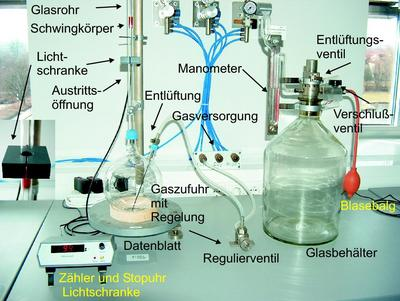
\includegraphics[scale=1.0]{aufbau.png}
 \caption{\label{fig:aufbau}Versuchsaufbau\protect\footnotemark}
\end{figure}
\footnotetext{https://lp.uni-goettingen.de/get/text/3639  Abb.3725}

\section{Auswertung}
\label{sec:auswertung}

\subsection{Rüchardt}
Vor dem Versuch wurde der Umgebungsdruck im Raum gemessen. Dieser betrug $p_0=1004,1\hecto\pascal$. Außerdem wurden folgende Werte von dem Versuchsaufbau abgelesen: $M=4,88\gramm$ (Masse des schwingenden Körpers), $d=9,97\milli\meter$ (Rohrdurchmesser) und $V=2300\centi\meter^3$ (Kolbenvolumen). Der Fehler des Umgebungsdrucks ist klein und kann daher vernachlässigt werden. Die abgelesenen Wert waren ohne Fehlerangabe und werden daher als exakt angenommen.\\

Aus diesen Werten berechnet sich der Druck im Kolben mit Formel \ref{eq:1} und $A=\pi\cdot (d/2)^2$ zu $p=101024\pascal$. Um die effektive Masse des schwingenden Körpers zu bestimmen muss die Masse der mitschwingenden Luftsäule $m_L=hA\rho_L$ beachtet werden. Dabei ist $\rho_L=1,225\kilogramm/\meter^3$ die Luftdichte bei $15\degree\celsius$ und $h=11,5\centi\meter$ die Höhe der Luftsäule. Die effektive Masse ist dann
\begin{align*}
m_{eff}=m+m_L=4,89\cdot10^-3\kilogramm.
\end{align*}
Nun kann aus denn Messwerten und der Formel
\begin{align*}
\kappa=\frac{c_p}{c_V}=\frac{64\cdot m_{eff}\cdot V}{T^2\cdot p\cdot d^4}
\end{align*}
für jede Messung der Adiabatenexponent bestimmt werden. Die gewichteten Mittelwerte der Ergebnisse sind in Tabelle \ref{tab:ruechardt} zusammen mit dem Fehler aufgeführt. Zur Fehlerberchnung wurde davon ausgegangen, dass die Stopuhr mit einem systematischen Fehler $\sigma_T$ von maximal 3\% behaftet ist. Der Gesamtfehler ergibt sich dann durch Fehlerfortpflanzung zu
\begin{align*}
\sigma_\kappa=\sqrt{\left(\frac{\partial\kappa}{\partial T}\right)^2\sigma_T^2}=\sqrt{\left(\frac{2\cdot64\cdot m\cdot V}{T^3\cdot p \cdot d^4}\right)^2\sigma_T^2}.
\end{align*}

\begin{table} [H]
\centering
\begin{tabular}{|r|c|c|c|c|} \hline
    Gas & $\kappa$ & $\sigma_\kappa$ & $f$ & $\sigma_f$ \\ \hline
    Luft & 1,28& 0,02 & 7,14 &  0,14\\
    $\rm{CO_2}$ & 1,22& 0,02 & 9,09 & 0,18 \\
    Arg & 1,53& 0,02 & 3,77 &  0,08 \\ \hline
 \end{tabular} 
 \caption{\label{tab:ruechardt}Ergebnisse nach Rüchardt}
\end{table}

Zum Schluss lassen sich die Freiheitsgrade mit Formel \ref{eq:2} berechnen
\begin{align*}
f=\frac{2}{\kappa-1}
\end{align*}
mit dem Fehler
\begin{align*}
\sigma_f=\sqrt{\left(\frac{\partial f}{\partial \kappa}\right)^2\sigma_\kappa^2}=\frac{2}{\left(k-1\right)^2}\sigma_\kappa.
\end{align*}
Die Ergebnisse sind ebenfalls in Tabelle \ref{tab:ruechardt} zu finden.




\subsection{Clement-Desormes}

Die Adiabatenexponente nach Clement-Desormes berechnte sich durch
\begin{align*}
\kappa=\frac{c_p}{c_V}=\frac{\Delta h_1}{\Delta h_1-\Delta h_2}
\end{align*}
mit dem Fehler
\begin{align*}
\sigma_\kappa=\sqrt{\left(\frac{\partial\kappa}{\partial h_1}\right)^2\sigma_{\Delta h_1}^2+\left(\frac{\partial\kappa}{\partial h_2}\right)^2\sigma_{\Delta h_2}^2}=\sqrt{\frac{\Delta h_2}{(\Delta h_2-\Delta h_1)^2}\sigma_{\Delta h_1}+\frac{\Delta h_1}{(\Delta h_1-\Delta h_2)^2}\sigma_{\Delta h_2}}
\end{align*}
Die berechneten gewichteten Mittelwerte für die einzelnen Zeitintervalle sind in Tabelle \ref{tab:clement} aufgeführt. Der Ablesefehler wurde mit $\sigma_{\Delta h_1}=\sigma_{\Delta h_2}=1\milli\meter$ abgeschätzt. Insgesamt beträgt der gewichtete Mittelwert aus den Messdaten
\begin{align*}
\kappa=1,35\pm0,01.
\end{align*}

\begin{table} [H]
\centering
\begin{tabular}{|r|c|c|} \hline
    $T\,[s]$ & $\kappa$ & $\sigma_\kappa$ \\ \hline
    $0,1$ & 1,38& 0,03 \\
    $1,0$ & 1,38& 0,03\\
    $5,0$ & 1,3& 0,03\\ \hline
 \end{tabular} 
 \caption{\label{tab:clement}}
\end{table}
Nun soll noch der gewichtet Mittelwert von $\kappa$ für Luft aus den beiden Experimenten gebildet werden. Dieser berechnet sich zu
\begin{align*}
\kappa=\frac{\kappa_R/\sigma_{\kappa_R}^2+\kappa_C/\sigma_{\kappa_C}^2}{1/\sigma_{\kappa_R}^2+1/\sigma_{\kappa_C}^2}\pm\sqrt{\left(\frac{1}{\sigma_{\kappa_R}^2}+\frac{1}{\sigma_{\kappa_C}^2}\right)^{-1}}=1,34\pm0,02
\end{align*}


\section{Diskussion}
\label{sec:diskussion}
Der theoretische Wert des Adiabatenexpnenten von Luft liegt bei $\kappa=1,40$. Unser Ergebnis liegt zwar nicht in der Fehlertoleranz, weicht aber nur um weniger als 5\% von diesem Wert ab. Bei der Berechnung nach Rüchardt fällt auf, dass die Werte des Adiabatenexpnenten für alle drei Gase deutlich unter dem theoretisch zu erwartenden Werten liegen. Daher liegt die Vermutung nahe, dass hir ein systematischer Fehler vorliegt. Dieser Fehler setzt sich in der Berechnung der Freiheitsgrade fort, was deren Abweichungen erklärt. 



\newpage
\section*{Anhang}

\begin{table} [H]
\centering
\begin{tabular}{|c|c||c|c|c|} \hline
    Messung & Perioden & Luft & CO$_2$ & Ar \\\hline
    $1 $&$ 1 $&$ 751 $&$ 768 $&$ 685$ \\
    $2 $&$ 1 $&$ 750 $&$ 769 $&$ 687$ \\
    $3 $&$ 1 $&$ 749 $&$ 770 $&$ 686$ \\
    $4 $&$ 1 $&$ 751 $&$ 769 $&$ 687$ \\
    $5 $&$ 1 $&$ 749 $&$ 771 $&$ 687$ \\
    $6 $&$ 1 $&$ 749 $&$ 770 $&$ 687$ \\
    $7 $&$ 1 $&$ 751 $&$ 771 $&$ 685$ \\
    $8 $&$ 1 $&$ 751 $&$ 770 $&$ 686$ \\
    $9 $&$ 1 $&$ 749 $&$ 771 $&$ 686$ \\
    $10 $&$ 1 $&$ 750 $&$ 768 $&$ 686$ \\
    \hline
    $1 $&$ 10 $&$ 7512 $&$ 7698 $&$ 6862$ \\
    $2 $&$ 10 $&$ 7520 $&$ 7702 $&$ 6864$ \\
    $3 $&$ 10 $&$ 7524 $&$ 7701 $&$ 6866$ \\
    \hline
    $1 $&$ 20 $&$ 15012 $&$ 15407 $&$ 13735$ \\
    $2 $&$ 20 $&$ 15007 $&$ 15412 $&$ 13737$ \\
    $3 $&$ 20 $&$ 15028 $&$ 15419 $&$ 13734$ \\
    \hline
    $1 $&$ 50 $&$ 37540 $&$ 38542 $&$ 34350$ \\
    $2 $&$ 50 $&$ 37560 $&$ 38533 $&$ 34345 $\\
    $3 $&$ 50 $&$ 37567 $&$ 38573 $&$ 34352 $\\
    \hline
    $1 $&$ 100 $&$ 75176 $&$ 77110 $&$ 68726$ \\
    $2 $&$ 100 $&$ 75192 $&$ 77138 $&$ 68722$ \\
    $3 $&$ 100 $&$ 75216 $&$ 77157 $&$ 68544$ \\
    \hline
 \end{tabular} 
 \caption{\label{tab:}Messwerte in Millisekunden für den Versuch nach Rüchardt}
\end{table}


\begin{table} [H]
\centering
\begin{tabular}{|c|c|c|} \hline
    Öffnungszeit & $\Delta h_1$ [\milli\meter] & $\Delta h_2$ [\milli\meter]  \\			\hline
	$0,1$ & $48$ & $14$ \\
	$0,1$ & $32$ & $8$\\
	$0,1$ & $31$ & $10$\\
    \hline
	$1,0$ & $54$ & $14$\\
	$1,0$ & $40$ & $10$\\
	$1,0$ & $35$ & $11$\\
    \hline
	$5,0$ & $44$ & $12$\\
	$5,0$ & $32$ & $7$\\
	$5,0$ & $37$ & $7$\\
    \hline
 \end{tabular} 
 \caption{\label{tab:}Messwerte für den Versuch nach Clement-Desormes}
\end{table}





%\begin{wraptable}{r}{5cm}
%\centering
%\begin{tabular}{r|l}
% \end{tabular} 
% \caption{\label{tab:}}
%\end{wraptable}

%\begin{table}
%\centering
%\begin{tabular}{r|c}
%    
% \end{tabular} 
% \caption{\label{tab:}}
%\end{table}




\end{document}
